\documentclass[a4paper]{article}

\usepackage[inner=2.0cm,outer=2.0cm,top=2.5cm,bottom=2.5cm]{geometry}
\usepackage{amsthm}
\usepackage{amssymb}
\usepackage{amsmath}
\usepackage{hyperref}
\usepackage{graphicx}
\usepackage[capitalize]{cleveref}
\usepackage{multicol}
\setlength\parindent{0pt}
\setlength\parskip{0.5em}
%%%%%%%%%%%%%%%%%%%%%%%%

\usepackage[utf8]{inputenc}
\usepackage{tikz}
\usetikzlibrary{shapes.geometric, arrows}

\tikzstyle{startstop} = [rectangle, rounded corners, minimum width=3cm, minimum height=1cm,text centered, draw=black, fill=red!30]
\tikzstyle{io} = [trapezium, trapezium left angle=70, trapezium right angle=110, minimum width=3cm, minimum height=1cm, text centered, draw=black, fill=blue!30]
\tikzstyle{process} = [rectangle, minimum width=3cm, minimum height=1cm, text centered, text width=3cm, draw=black, fill=orange!30]
\tikzstyle{decision} = [diamond, minimum width=3cm, minimum height=1cm, text centered, draw=black, fill=green!30]
\tikzstyle{arrow} = [thick,->,>=stealth]
%%%%%%%%%%%%%%%%%%%%%%%%%%%%%
%%%%%%%%%%%%%%%%%%%%%%%%%%
\usepackage{listings}
\usepackage{xcolor}

\definecolor{codegreen}{rgb}{0,0.6,0}
\definecolor{codegray}{rgb}{0.5,0.5,0.5}
\definecolor{codepurple}{rgb}{0.58,0,0.82}
\definecolor{backcolour}{rgb}{0.95,0.95,0.92}

\lstdefinestyle{mystyle}{
    backgroundcolor=\color{backcolour},   
    commentstyle=\color{codegreen},
    keywordstyle=\color{magenta},
    numberstyle=\tiny\color{codegray},
    stringstyle=\color{codepurple},
    basicstyle=\ttfamily\footnotesize,
    breakatwhitespace=false,         
    breaklines=true,                 
    captionpos=b,                    
    keepspaces=true,                 
    % numbers=left,                    
    numbersep=5pt,                  
    showspaces=false,                
    showstringspaces=false,
    showtabs=false,                  
    tabsize=2
}
\lstset{style=mystyle}
%%%%%%%%%%%%%%%%%%%
\usepackage{biblatex} %Imports biblatex package
\addbibresource{References.bib} %Import the bibliography file
% %%%%%%%%%%%%%%%%%%%
% \usepackage{titlesec}
% \usepackage{textcase,relsize}

% \def\myFBRSC#1{{\larger[3]{\MakeTextUppercase{#1}}}\scshape }
% \DeclareRobustCommand{\FirstBigRestSmallCaps}[1]{\myFBRSC #1}

% \titleformat{\section}%
% {\normalfont\Large}{\thesection}{1em}{\FirstBigRestSmallCaps}
% %%%%%%%%%%%%%%%%%%%%
% ==== Environments ====
% Not recommended to change the environment definitions.
\newcounter{solution}
\newcounter{subsolution}[solution]
\newcommand{\solution}{\section*{Solution \stepcounter{solution}\arabic{solution}}}
\newcommand{\subsolution}{\paragraph{(\protect\stepcounter{subsolution}\arabic{subsolution})}}
\newtheorem{claim}{Claim}[solution]

% ==== Custom Commands ====
% Not recommended to change the definitions of existing commands.
\newcommand{\homeworktitle}[2]{\begin{center}
    \framebox{\begin{minipage}{0.9\textwidth}
        \textbf{Project Elective} \hspace*{\fill} \today
        \vspace{2mm}
        \begin{center}
            {\Large #2}
        \end{center}
        \vspace{2mm}
        \text{Anurag Singh Naruka (IMT2020093)} \hspace*{\fill} #1
    \end{minipage}}
\end{center}
\vspace*{4mm}}

% ==== Custom Math Commands ====
% A few macros we've used to get you started.
\newcommand{\set}[1]{\ensuremath{\{ #1 \}}}
\newcommand{\setsize}[1]{\ensuremath{| #1 |}}

\begin{document}
% Replace the name, rollnumber and title of the document.
\homeworktitle{ Instructor: Prof. Amit Chattopadhyay
  \\  Ujjwal Agarwal (IMT2020128) }{Reeb Graph Computation And Visualization}
\textbf{Abstract}: This is the summary of our understanding of the research paper "Output-Sensitive Construction of Reeb Graphs" by Harish Doraiswamy and Vijay Natarajan \cite{Vijay}. Here we will discuss the necessary definitions and working of the algorithm proposed in this paper with its key aspects. We will also discuss how we visualize the obtained Reeb Graph in a 3-D space as a contour tree Radial Tree graph layout and a tool made to interact with the reeb graph for analysing it.
 
\begin{multicols}{2}
\section{Introduction}
A Reeb graph is a mathematical object reflecting the evolution of the level sets of a real-valued function on a manifold. The Reeb graph of a scalar function is obtained by mapping each connected component of its level sets to a point. For 2 manifolds Cole-Mclaughlin et al proposed an algorithm that efficiently stores and manipulates the  connected components of level sets that lead to fast construction of Reeb graph in O(nlogn) by maintaining the level sets using dynamically balanced
search trees. There are other efficient Reeb graph computation techniques, however they make certain assumptions based on the graphs.\\\\
For higher manifolds or non-manifold, Doraiswamy and Natarajan stored the connected components of level sets using dynamic connectivity data structures resulting in an algorithm that computes the Reeb graph of a scalar function. It presents an efficient two-step algorithm for computing the Reeb graph of a piecewise-linear (PL) function in O(n + l +t logt) time, where n is the number of triangles in the input mesh, t is the number of critical points of the function, and l is the total size (number of edges) of all critical level sets.\\\\

\includegraphics[width=1\linewidth]{reeb-graph-torus.png}

\section{BACKGROUND}
\subsection{Level Set}
 A level set of a real-valued function f of n real variables is a set where the function takes on a given constant value c, that is:

${\displaystyle L_{c}(f)=\left\{(x_{1},\ldots ,x_{n})\mid f(x_{1},\ldots ,x_{n})=c\right\}~}$\\

\subsection{Contour Tree}
A contour is a single connected component of the level set.The contour tree \cite{CT} is a loop-free Reebgraph that tracks the evolution of contours. Each leaf node is a minimum or
maximum; each interior node is a saddle; each edge represents a set of adjacent contours with isovalues between the
values of its two ends. There is a one-to-one mapping from a point in the contour tree (at a node or in an edge) to a contour of the scalar field.

\subsection{Morse Function}
A function f : M $\rightarrow$ R is a Morse function iff the following conditions
are met:\\
\begin{enumerate}
    \item None of f’s critical points are degenerate.
    \item No two of f’s critical points share the same function value.
\end{enumerate}
   


\subsection{Radial Tree Layout}
The Radial-Tree Layout arranges nodes in a circular layout, positioning the root node at the center of the graph and the child nodes in a circular fashion around the root. Sub-trees formed by the branching of child nodes are located radically around the child nodes. In this paper we are visualizing the side view of Radial Tree.


\section{Reeb Graph Algorithm}
This algorithm computes a Reeb graph of a piecewise linear function \textit{ƒ} defined on a 3-manifold.
This consist of two steps: firstly we will locate all the critical points in the domain and sort them based on their function value and then identify pairs of critical points that define \textbf{cylinders} and insert the corresponding arc in Reeb graph.\\\\
\textbf{Cylinders:} Collection of mesh triangles. A cylinder bounded by two critical level set components is represented by triangles that contain the intermediate level set components.\\\\
As discussed above Reeb graph is obtained by mapping each connected component of its level sets to a point. Here nodes of Reeb Graph will be mapped to components of critical level sets and arcs will be mapped to equivalence classes of regular level set components.\\\\
A dual graph is introduced to store triangle adjacencies and helps implicitly track level set components of individual cylinders. This graph is a  directed graph GLS (V,E), called the LS-graph. It has nodes V = \{$t_{1}$,$t_{2}$,...,$t_{n}$\} corresponds to the n triangles \{$T_{1}$,$T_{2}$,...,$T_{n}$\} in the input mesh. 

\includegraphics[width=1\linewidth]{fig_1.png} \\
In the given triangulation of the input mesh, there can only be six possible configurations of adjacent triangles. The LS-graph contains an edge from $t_{i}$ to $t_{j}$ in all cases except the forbidden configuration in (f). Edges in the graph are directed toward the node with a higher cost

\includegraphics[width=1\linewidth]{fig_2.png}\\\\  
\textbf{Connecting the critical points:}
Here of the two-step algorithm computing the Reeb graph of the height function defined on a solid 2-torus.
This model has ten critical points, including two minima, two maxima, and six saddle points. The critical points are first sorted in increasing order of function value. Let $c_1, c_2,..., c_{10}$ be the ten critical points in sorted order. Beginning
with a triangle in the upper star of $c_1$, the algorithm traces the green cylinder to reach $L_3$ and inserts ($c_1, c_3$) into the
Reeb graph. Then the search from $c_2$ also reaches $L_3$, but a different component as compared to the previous trace. So ($c_2, c_3$) is inserted into the Reeb graph. The upper star of $c_4$ has two components. A search is initiated from each
component to obtain the two parallel arcs ($c_4, c_5$) of the Reeb graph. While tracing the cylinder from $c_6$, the search procedure reaches a triangle with cost greater than f7 that does not belong to $L_7$. The search procedure next reaches
$L_$8 and the arc ($c_6, c_8$) is inserted into the Reeb graph.The Reeb graph of the input function is computed after all critical points are processed.

\section{Implementation}
\subsection{Mesh Simplification}
We then explored some mesh simplification tools in order to remove unnecessary processing.
Mainly we found two tools -\\ 1. \textbf{Blender}\\ 2. \textbf{ZBrush} \\
In blender we were able to perform mesh simplification after following some tutorials, but the process sometimes failed due to unknown reasons. \\
Zbrush on the other hand, was much easier to use. ZBrush uses \textbf{quadratic decimation} to perform mesh simplification which does not affect or change the topology. Hence was ideal for our use. 
\begin{center}
    
\includegraphics[width=0.8\linewidth ]{socket-pic.jpeg}\\\\
\includegraphics[width=0.8\linewidth ]{socket-simplified-pic.jpeg}\\\\
\end{center}


\subsection{Conversion of files}
We have been working with different types of files. For making the reeb graph we need to input the file in OFF format. We have written a python program to convert gts to off format and for other formats you can use this \href{https://imagetostl.com/convert/file/obj/to/off}{link}.\\

Now talking about off file format.
\begin{itemize}
    \item Optional first line containing "OFF".
    \item Next line specifies the no. of vertices (nv) followed by the number of triangles (nt) (space seperated)
    \item The next nv lines contains x y z f where x, y & z specify the co-ordinates of the vertex and f specifies the function value. 
    \item The next nt lines has 3 v1 v2 v3 where v1, v2 and v3 are the vertex indices of the vertices that form the triangles.
\end{itemize} 
In the third point as mentioned above we have to give functional value that will correspond to the function based on which the algorithm will be computing critical points and compute a reeb graph. Consider that function as a height function on z-axis, so in our off file format the nv lines will look like x y z z(this z for function value) then algorithm will compute a reeb graph based on the given height function. We have written a file named append\_height\_z to give a functional value to any off file(available on github). \textbf{These functional value can also take scaler values.}

\subsection{Observations from Reeb Graph file}
Now we have the off file with some functional value we will give this input to our algorithm and get the output file(.rg file) which basically is our reeb graph.\\\\

\textbf{
[.rg file for Torus]\\}

\begin{lstlisting}
4 4
0 -54.36 MINIMA
13 -32.1389 SADDLE
150 3.5702 SADDLE
145 25.7913 MAXIMA
0 13 
13 150 
150 145 
13 150 

\end{lstlisting}



In first line of the .rg file there are two things 1st number is the number of critcal points say M and 2nd number denotes the number of edges(or arcs) say N in the Reeb graph. Next following M lines give three things, indices of the critical points followed by function value and then the type of critical point. And there are N more lines which tell us about the edges (or arcs) between the two vertices.

From the above example of the .rg file of Torus, We can see that the vertex 13 and 150 are SADDLES and there is a connection between these two SADDLES which is repeated (3rd last line and last line of Example) this tells us that there are two arcs between vertex 13 and 150 which should be there as it is a Torus. So for making the loops in Radial Tree Layout if a connection is repeated we will add a loop between these points seprately.\\
\newline
\textbf{
All critical points will be either minima or maxima will exactly be a part of one edge in the graph which means that if me make a graph from these N connections(edges or arcs) the degree of all minima or maxima will be one i.e all these points will be the leaf nodes of the graph and all other nodes (except the root node) will be a SADDLE.
}
\subsection{Radial Tree Layout Of Reeb Graph}
Now as we have the .rg file we can use any layout scheme and visualize it. Here we will use the Radial Tree layout to visualize the Reeb graph.Radial Tree layout scheme is not easy because of the loops present in Reeb Graph.We overcome this difficulty
by designing a four step layout scheme:
\begin{enumerate}
    \item Extract a spanning contour tree of the Reeb graph.
    \item Compute a branch decomposition of this spanning
tree.
    \item Use a Radial Tree layout scheme to embed the spanning
tree in 3D
    \item Add the non-tree arcs to the layout.
    
\end{enumerate}
We have written a layout.sh file to run the LayoutReebGraph.java files that calls the four functions as mentioned above.We will input our Reeb Graph file to the layout.sh and we will get a text file which is Radial Tree Layout for the given off file.\\\\
\textbf{Output File of Radial Tree Layout for Torus}\\
\begin{lstlisting}
0 0.0 -2.0 0.0
13 0.0 -0.89104235 0.0
150 0.0 0.89104223 0.0
145 0.0 2.0 0.0
\end{lstlisting}

The layout file will have all the critical points and its location (x y z co-ordinate of that point).


\subsection{Visualization Of Radial Tree Layout}
The Radial Tree Layout has been viasualized using the Three.js Library which is an application programming interface used to create and display animated 3D computer graphics in a web browser using WebGL. \\\\
Here we create a tool to interact with the reeb graph of a manifold to better understand and analyze it. The reeb graph helps us to visualize the critical points, red for maxima, green for saddle and blue for minima. The edges represents all the regular points of the shape. \\\\
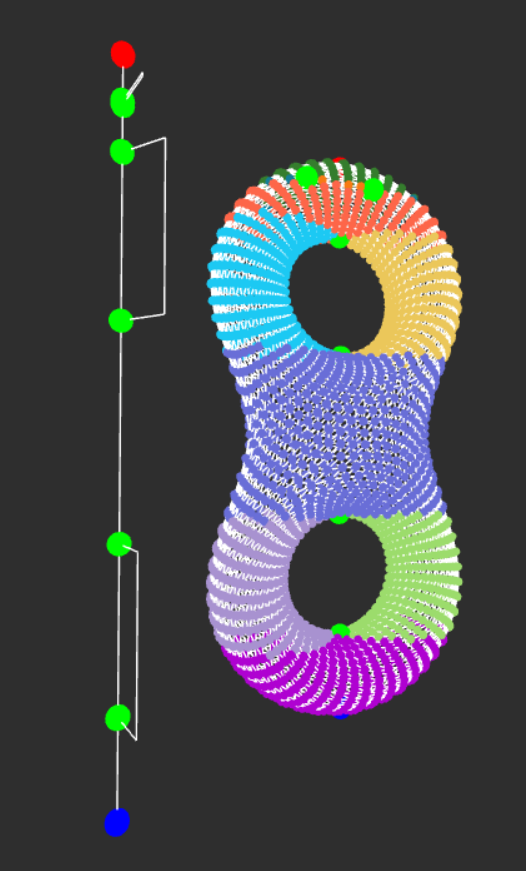
\includegraphics[width=1\linewidth]{double-torus-all-lvl-sets.png}

\subsection{Examples}
In this tool when an edge of the reeb graph is hovered over with the pointer then the corresponding points of the level set are highlighted on the mesh of the manifold.\\\\
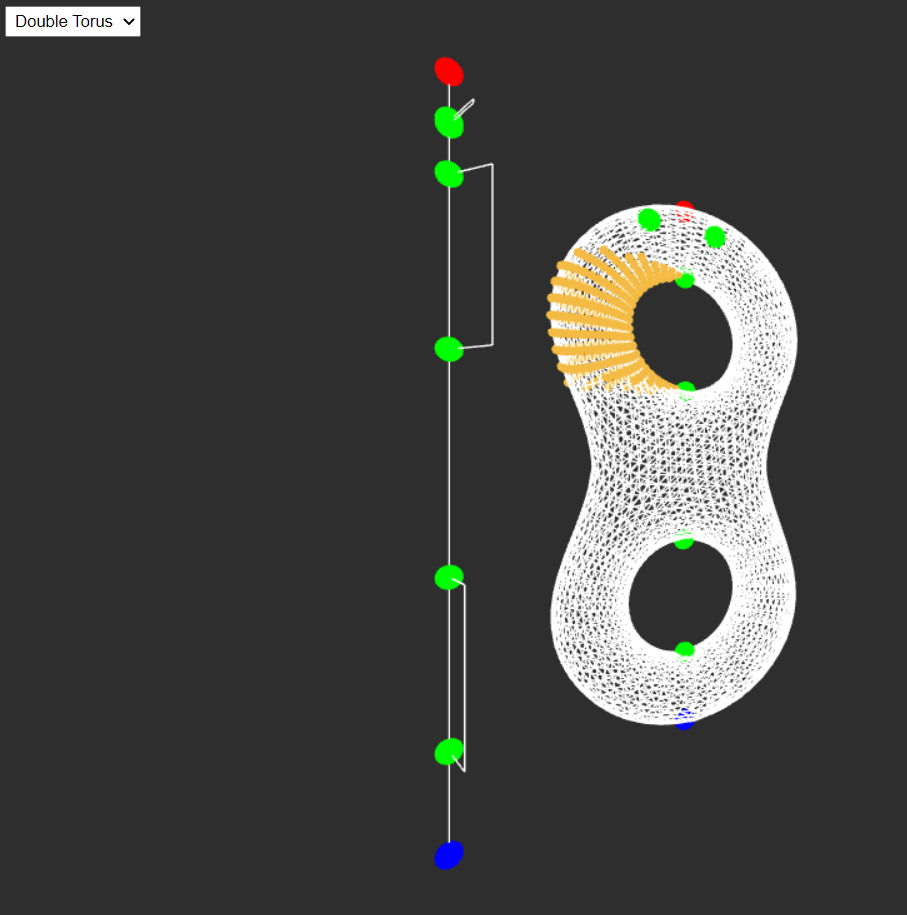
\includegraphics[width=0.85\linewidth]{double-torus.png} \\
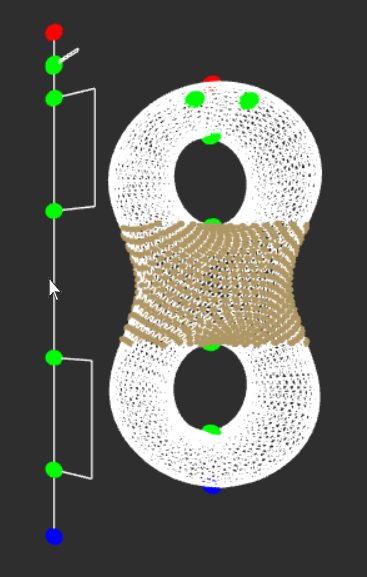
\includegraphics[width=1\linewidth]{double-torus-hover-middle.png}

% \section{Flow}
% \begin{center}
    
% \begin{tikzpicture}[node distance=2cm]

% \node (start) [startstop] {Start};
% \node (in1) [io, below of=start] { .off file };
% \node (pro1) [process, below of=in1] {.rg file};
% \node (pro2) [process, below of=pro1] {.txt file (layout file)};
% \node (pro3) [process, below of=pro2] {Visualize the .txt file};
% \node (stop) [startstop, below of=pro3] {Stop};

% \draw [arrow] (start) -- (in1);
% \draw [arrow] (in1) -- (pro1);
% \draw [arrow] (pro1) -- (pro2);
% \draw [arrow] (pro2) -- (pro3);
% \draw [arrow] (pro3) -- (stop);


% \end{tikzpicture}
% \end{center}
\printbibliography
\end{multicols}
\end{document}
